%%%%%%%%%%%%%%%%%%%%%%%%%%%%%%%%%%%%%%%%%
% Jacobs Landscape Poster
% LaTeX Template
% Version 1.0 (29/03/13)
%
% Created by:
% Computational Physics and Biophysics Group, Jacobs University
% https://teamwork.jacobs-university.de:8443/confluence/display/CoPandBiG/LaTeX+Poster
% 
% Further modified by:
% Nathaniel Johnston (nathaniel@njohnston.ca)
%
% This template has been downloaded from:
% http://www.LaTeXTemplates.com
%
% License:
% CC BY-NC-SA 3.0 (http://creativecommons.org/licenses/by-nc-sa/3.0/)
%
%%%%%%%%%%%%%%%%%%%%%%%%%%%%%%%%%%%%%%%%%

%----------------------------------------------------------------------------------------
% PACKAGES AND OTHER DOCUMENT CONFIGURATIONS
%----------------------------------------------------------------------------------------
  \documentclass[final]{beamer}

  \usepackage[scale=1.2]{beamerposter} % Use the beamerposter package for laying out the poster
  \usepackage{mathtools,amsmath}

  \usetheme{confposter} % Use the confposter theme supplied with this template
  \setbeamercolor{block example title}{fg=white,bg=calblue}
  \setbeamercolor{block title}{fg=calblue,bg=white} % Colors of the block titles
  \setbeamercolor{block body}{fg=black,bg=white} % Colors of the body of blocks
  \setbeamercolor{block alerted title}{fg=white,bg=calblue!70} % Colors of the highlighted block titles
  \setbeamercolor{block alerted body}{fg=black,bg=calblue!10} % Colors of the body of highlighted blocks
  \setbeamertemplate{itemize item}[triangle]
  \setbeamertemplate{caption}[numbered]
  % Many more colors are available for use in beamerthemeconfposter.sty

  %-----------------------------------------------------------
  % Define the column widths and overall poster size
  % To set effective sepwid, onecolwid and twocolwid values, first choose how many columns you want and how much separation you want between columns
  % In this template, the separation width chosen is 0.024 of the paper width and a 4-column layout
  % onecolwid should therefore be (1-(# of columns+1)*sepwid)/# of columns e.g. (1-(4+1)*0.024)/4 = 0.22
  % Set twocolwid to be (2*onecolwid)+sepwid = 0.464
  % Set threecolwid to be (3*onecolwid)+2*sepwid = 0.708

  \newlength{\sepwid}
  \newlength{\onecolwid}
  \newlength{\twocolwid}
  \newlength{\threecolwid}
  \setlength{\paperwidth}{48in} % A0 width: 46.8in
  \setlength{\paperheight}{36in} % A0 height: 33.1in
  \setlength{\sepwid}{0.024\paperwidth} % Separation width (white space) between columns
  \setlength{\onecolwid}{0.22\paperwidth} % Width of one column
  \setlength{\twocolwid}{0.464\paperwidth} % Width of two columns
  \setlength{\threecolwid}{0.708\paperwidth} % Width of three columns
  \setlength{\topmargin}{-0.5in} % Reduce the top margin size
  %-----------------------------------------------------------

  \usepackage{graphicx}  % Required for including images
  \usepackage{booktabs} % Top and bottom rules for tables
  \usepackage{apacite}
  \usepackage{wrapfig}
  \usepackage{amssymb,amsmath,amsthm,amsfonts}
  \usepackage{tikz}
  \usepackage{caption}
  \usepackage{listings}
  \usepackage{fancyvrb}
  \captionsetup{font=normalsize, labelfont=normalsize}


\title{Mouselab-MDP: A new paradigm for tracing how people plan}
\author{Frederick Callaway, Falk Lieder, Paul M. Krueger, and Thomas L. Griffiths}
\institute{University of California, Berkeley} % Institution(s)

\begin{document}

% Logos
\addtobeamertemplate{headline}{}
{\begin{tikzpicture}[remember picture, overlay]
  \node [anchor=north east, inner sep=2cm]  at (current page.north east)
  {
\includegraphics[height=8cm]{berkeley.png}};
  \node [anchor=north west, inner sep=2cm]  at (current page.north west)
  {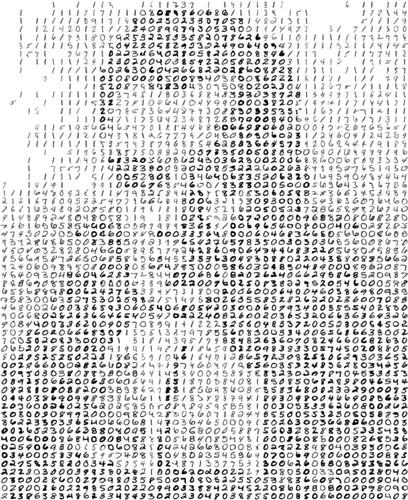
\includegraphics[height=8cm]{cocosci.jpg}};
\end{tikzpicture}}

\addtobeamertemplate{block end}{}{\vspace*{2ex}} % White space under blocks
\addtobeamertemplate{block alerted end}{}{\vspace*{2ex}} % White space under highlighted (alert) blocks
\setlength{\belowcaptionskip}{2ex} % White space under figures
\setlength\belowdisplayshortskip{2ex} % White space under equations

\begin{frame}[t, fragile] % The whole poster is enclosed in one beamer frame
\begin{columns}[t] % The whole poster consists of three major columns, the second of which is split into two columns twice
\begin{column}{\sepwid}\end{column} % Empty spacer column

%----------------------------------------------------------------------------------------
% CONTENT
%----------------------------------------------------------------------------------------

\begin{column}{\onecolwid} % Begin column 1
  \begin{block}{Motivation}\label{Motivation}
    Planning is a latent cognitive process that cannot be observed directly. This makes it difficult to study how people plan.
    To address this problem, we propose a new paradigm that provides experimenters with a timecourse of participant attention to information in the task environment.
  \end{block}

  % \begin{alertblock}{Key findings}\label{key-findings}
  %   \textbf{Sparse pseudo-rewards} can
  %   \begin{itemize}
  %     \item lead to \textbf{optimal behavior} in a \textbf{limited-depth planner}.
  %     \item induce \textbf{goal directed planning} in humans.
  %     \item \textbf{improve human decision making}.
  %   \end{itemize}
  % \end{alertblock}

  \begin{block}{Background}\label{Background}
    Planning is a fundamental aspect of higher-order cognition, and it has accordingly received much attention in cognitive psychology.
    Research on planning is complicated by the fact that we cannot directly observe the cognitive processes of planning.
    One approach to this problem is to design \emph{process tracing} paradigms that externalize some aspect of the cognitive process. \citeA{Payne1988} developed one such methodology for studying multi-alternative risky choice: the ``Mouselab'' paradigm.
    Thus, to apply the Mouselab process tracing method to planning, we simply replace the single decision with a Markov Decision Process (MDP), in which a participant must make a sequence of choices, each one affecting the choices that will be available in the future.
    Something about pruning?
  \end{block}

  \begin{block}{Usage}\label{usage}
    \begin{Verbatim}[fontsize=\small]
    "graph": {
      "0_3": {
        "right": [9, "1_3"]
      },
      "3_3": {},
      "1_1": {
        "down": [-6, "1_2"],
        "right": [4, "2_1"]
      },
      "1_2": {
        "down": [3, "1_3"],
        "right": [-7, "2_2"]
      },
      ...
    }
    \end{Verbatim}
  \end{block}

\end{column} % End column 1
%------------------------------------------------------------------------------

\begin{column}{\sepwid}\end{column} % Empty spacer column
\begin{column}{\twocolwid} % Begin column 2

  \begin{figure}
    % \label{fig:paradigm}
    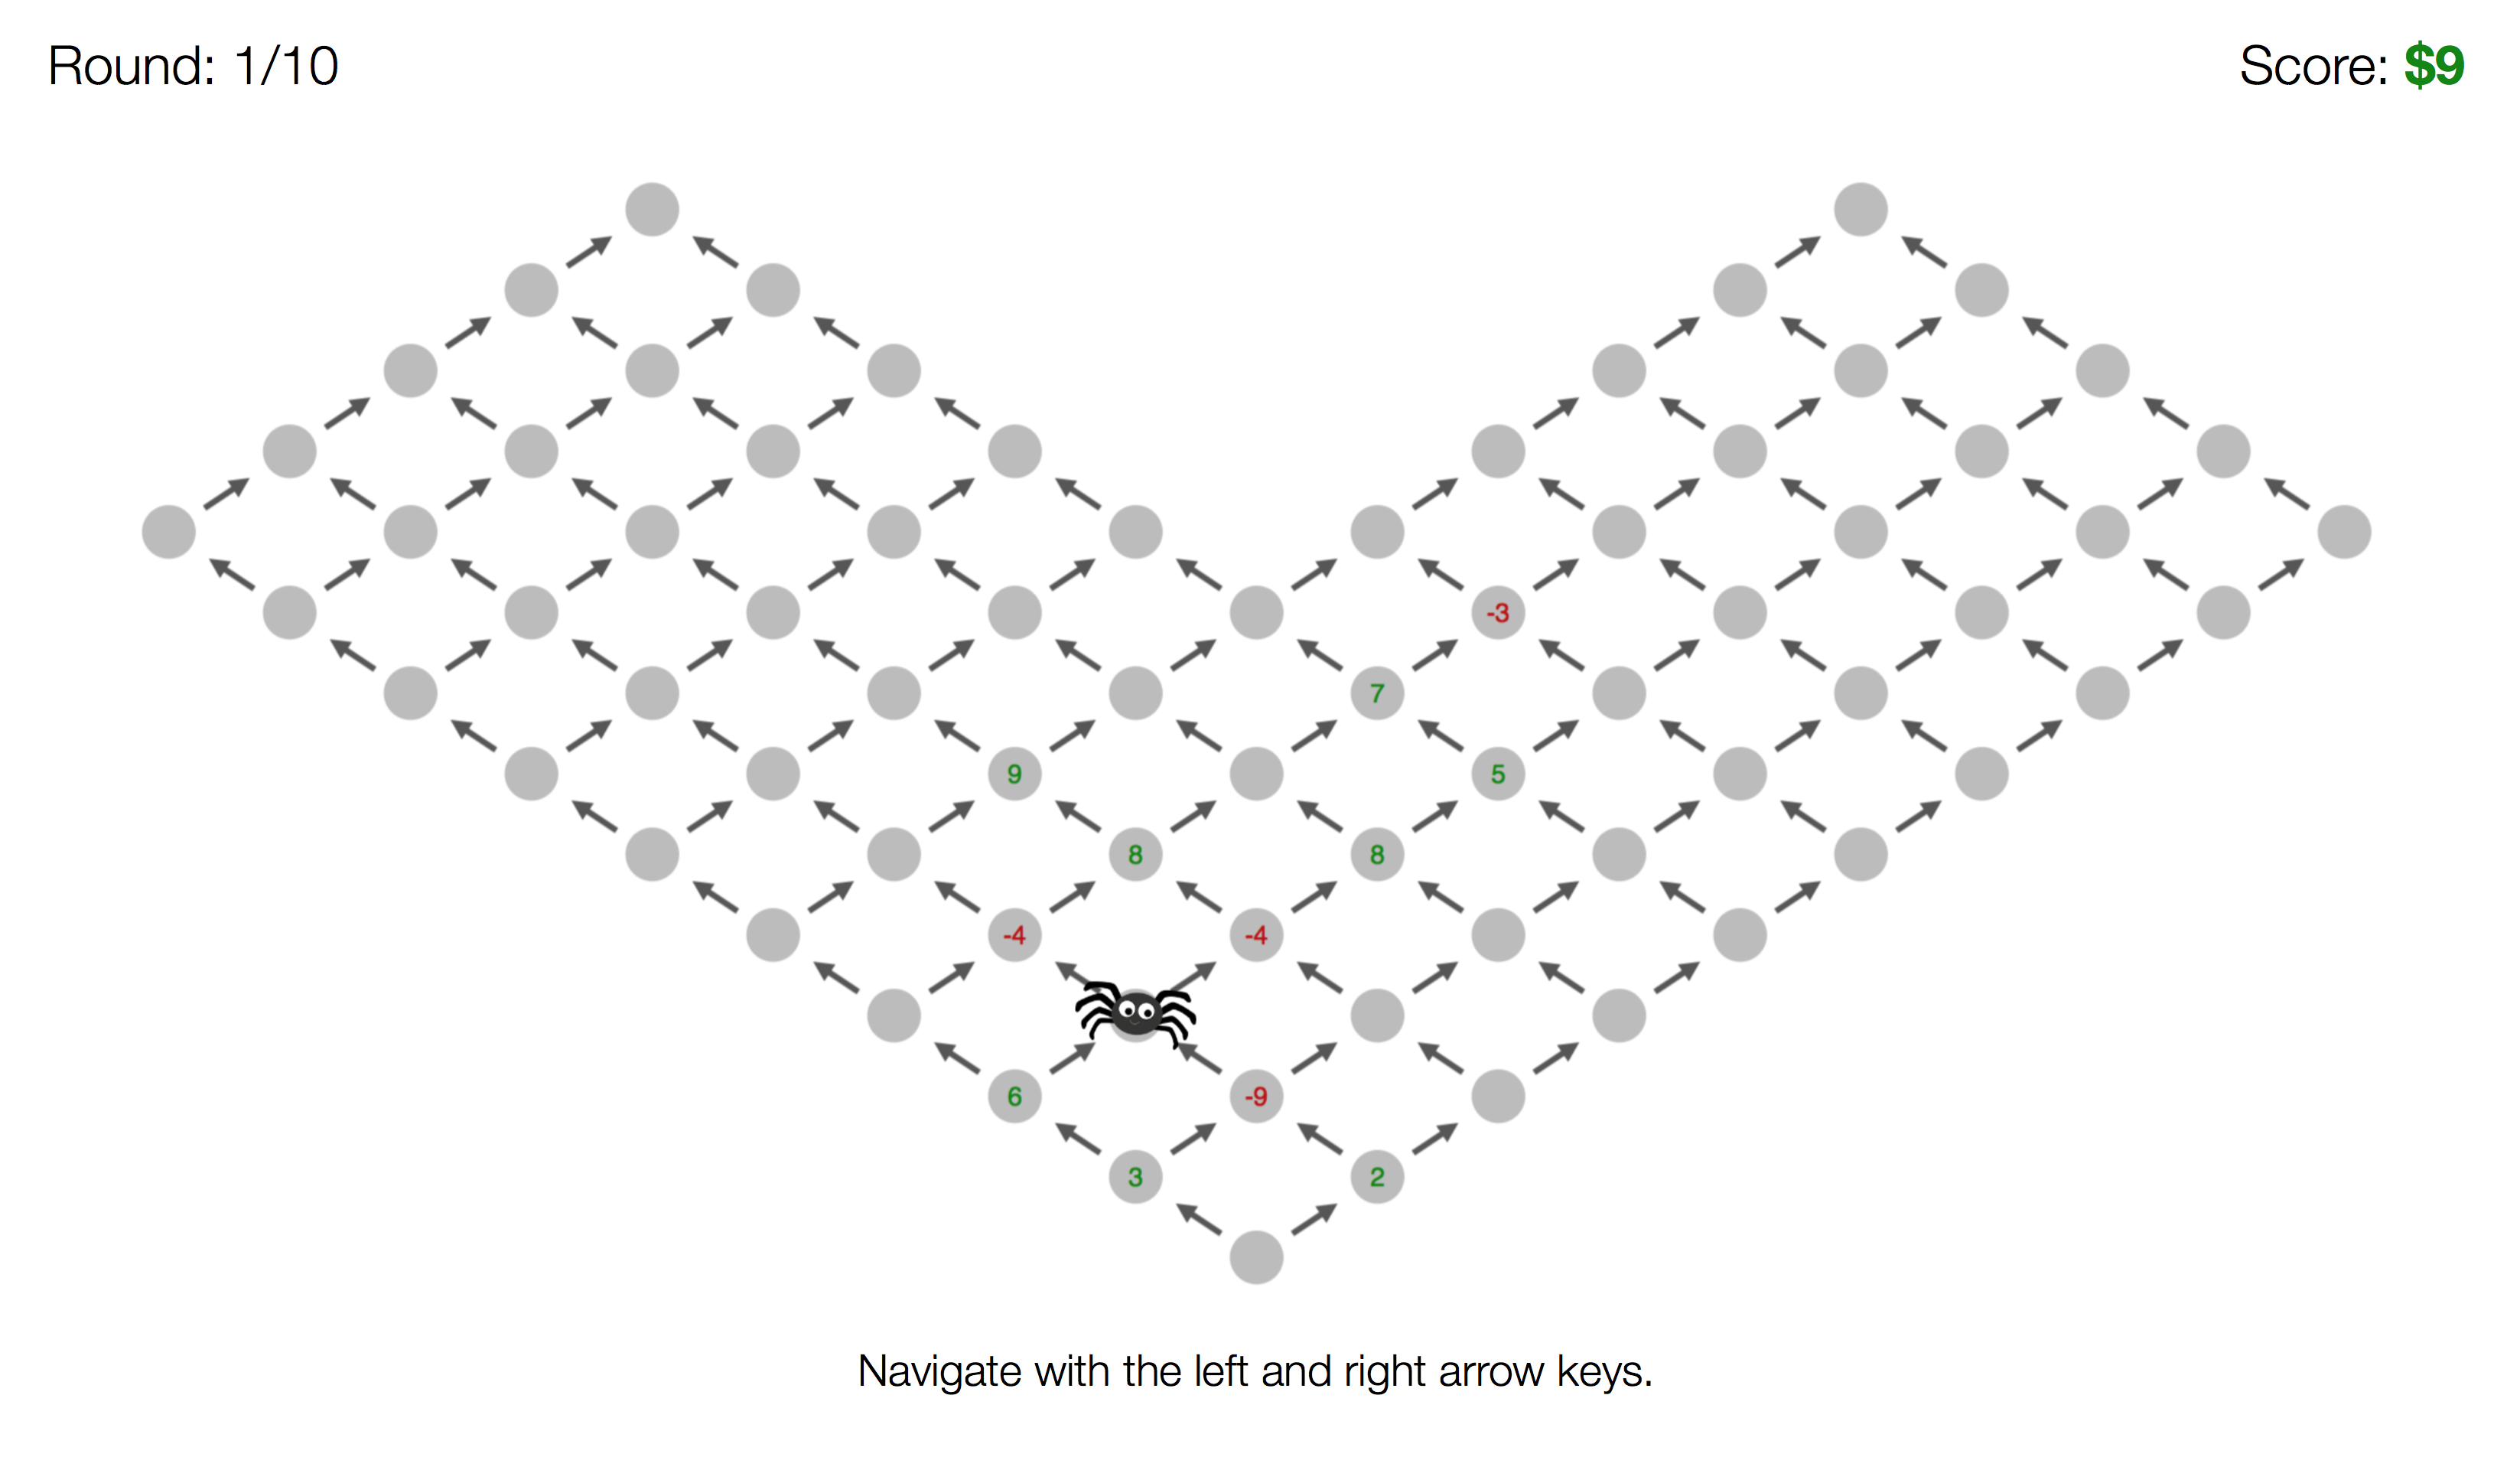
\includegraphics[width=0.9\linewidth]{figs/heart.png}
    % \captionsetup{width=0.9\linewidth}
    % \caption[first]{Web of Cash experimental interface.}
  \end{figure}

  % \vspace{-1cm}

  \begin{columns}[t,totalwidth=\twocolwid] % Split column 2 into 2.1 and 2.2
    
    \begin{column}{\onecolwid} % Begin column 2.1
      
      \begin{figure}
        % \label{fig:paradigm}
        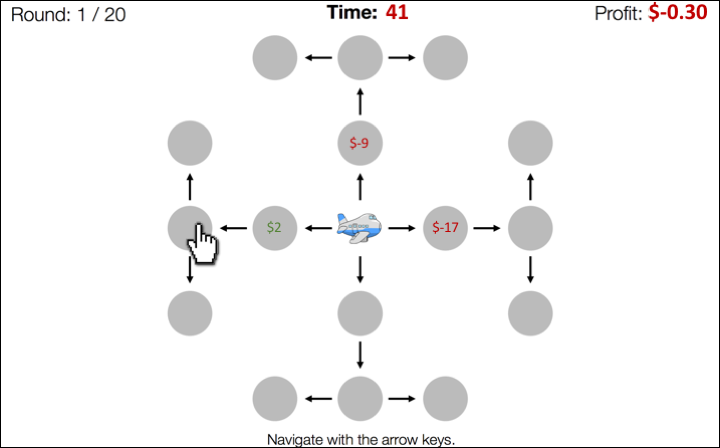
\includegraphics[width=0.9\linewidth]{figs/paradigm_illustration1.png}
        % \captionsetup{width=0.9\linewidth}
        % \caption[first]{Web of Cash experimental interface.}
      \end{figure}
      
      \begin{figure}
        % \label{fig:paradigm}
        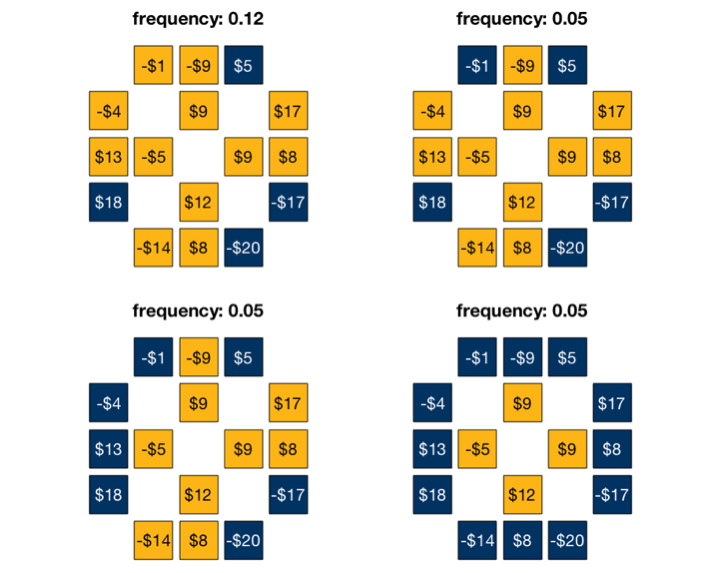
\includegraphics[width=0.9\linewidth]{figs/click_sets_trial4_noFB_small.png}
        % \captionsetup{width=0.9\linewidth}
        % \caption[first]{Web of Cash experimental interface.}
      
      \end{figure}
    \end{column} % End column 2.1

    \begin{column}{\onecolwid} % Begin column 2.2
     
      \begin{figure}
        % \label{fig:paradigm}
        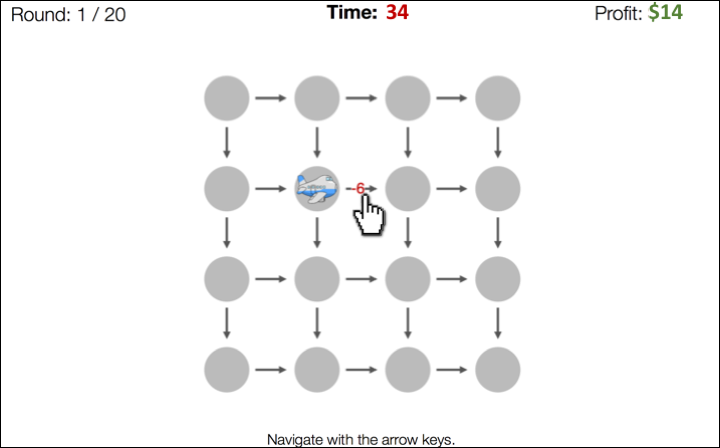
\includegraphics[width=0.9\linewidth]{figs/paradigm_illustration2.png}
        % \captionsetup{width=0.9\linewidth}
        % \caption[first]{Web of Cash experimental interface.}
      \end{figure}

      \begin{figure}
        % \label{fig:paradigm}
        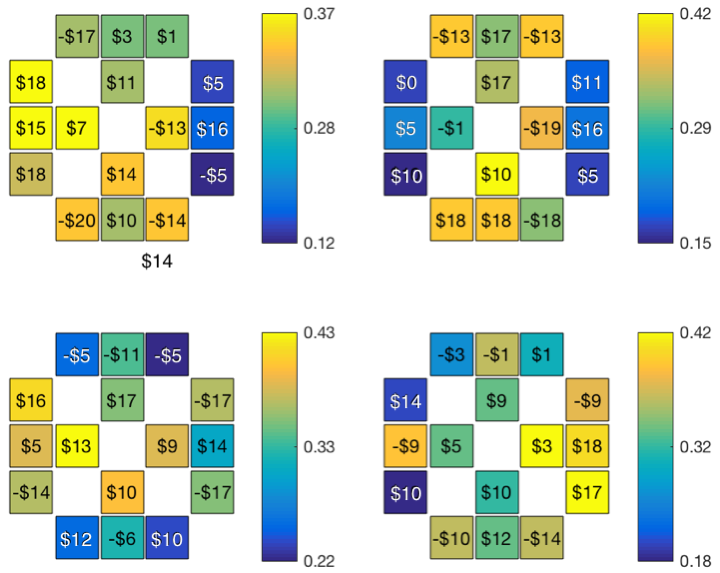
\includegraphics[width=0.9\linewidth]{figs/click_locations_noFB_before1stFlight_small.png}
        % \captionsetup{width=0.9\linewidth}
        % \caption[first]{Web of Cash experimental interface.}
      \end{figure}
    
    \end{column} % End column 2.2

  \end{columns}

\end{column} % End column 2
%------------------------------------------------------------------------------
\begin{column}{\sepwid}\end{column} % Empty spacer column
\begin{column}{\onecolwid} % Begin column 3

  \begin{block}{Experiment}\label{experiment}
  We used the Mouselab-MDP plugin for JsPsych. In each trial participants route an airplane from the center of the screen to one of eight final destinations via two intermediate locations (see Figure \ref{fig:Screenshots}a). We specified \texttt{stateLabels} as the rewards associated with the edge leading to each state. We set \texttt{stateDisplay} to `click' and `stateClickCost' to 0.10; thus participants could click on a state to reveal the reward for traveling to that state, at the price of $\$0.10$. Participants were required to spend at least $45$ seconds on every trial to prevent time cost from discouraging participants from clicking and planning. 

  \end{block}

  \begin{alertblock}{Results}\label{results}
    \begin{itemize}
      \item Something about pruning.
    \end{itemize}
  \end{alertblock}

  \begin{figure}
    % \label{fig:paradigm}
    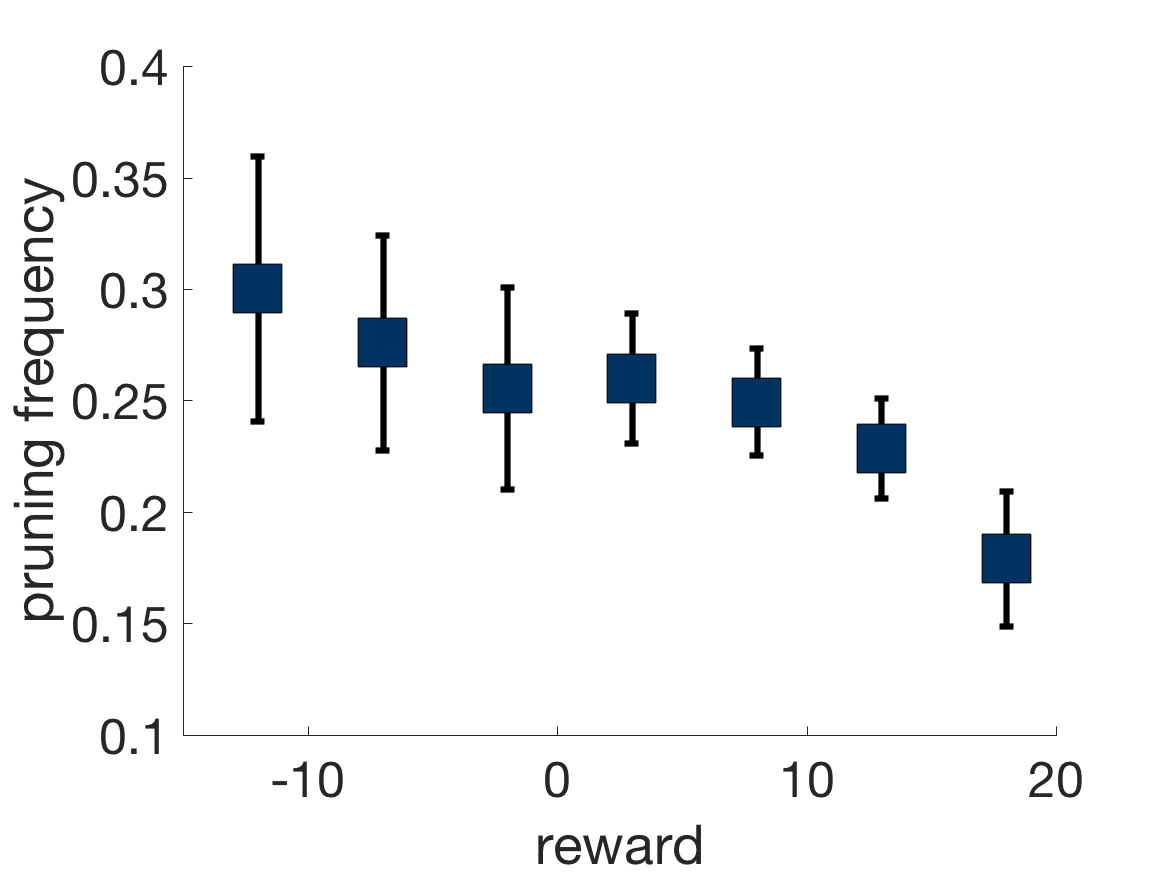
\includegraphics[width=0.9\linewidth]{figs/prunning_any_noFB.png}
    % \captionsetup{width=0.9\linewidth}
    % \caption[first]{Web of Cash experimental interface.}
  \end{figure}

  \begin{block}{References}\label{references}
    \bibliographystyle{apacite}
    \renewcommand{\bibliographytypesize}{\small}
    % \setlength{\bibleftmargin}{.05in}
    % \setlength{\bibindent}{-\bibleftmargin}
    \bibliography{references}
  \end{block}

  % \setbeamercolor{block title}{fg=red,bg=white} % Change the block title color

  % \begin{exampleblock}{Acknowledgements}
    \small{\rmfamily{\textbf{Funding}\; ONR MURI N00014-13-1-0341 and the Templeton World Charity Foundation.}}
  % \end{exampleblock}

  \begin{flushright}
    \texttt{fredcallaway@berkeley.edu}
  \end{flushright}

\end{column} % End column 3

\end{columns} % End of all the columns in the poster

\end{frame}

\end{document}
